\documentclass[tikz,crop,convert={density=300,outext=.png},border=0.0cm,width=18cm,height=7cm]{standalone}
%\documentclass[tikz,border=0.3cm]{standalone}
%\usepackage[left=2.2cm,right=2.2cm,top=2.5cm,bottom=2.0cm,a4paper]{geometry}
\usepackage{pgfplots}
\usepackage{amsmath}
\usepackage{physics}

\definecolor{one}{RGB}{0,68,27}
\definecolor{two}{RGB}{35,139,69}
\definecolor{three}{RGB}{153,216,201}
\pgfplotsset{compat=newest,
    %width=6cm,
    %height=3cm,
    scale only axis=true,
    max space between ticks=25pt,
    try min ticks=5,
    every axis/.style={
        axis y line=middle,
        axis x line=middle,
        axis line style={thick,->,>=latex, shorten >=-.3cm}
    },
      every axis plot/.append style={thick},
    tick style={black, thick},
}
\tikzset{
    semithick/.style={line width=0.8pt},
  }
\usetikzlibrary{shapes.geometric, arrows}  
\usepgfplotslibrary{groupplots}
\usepgfplotslibrary{dateplot}
\usetikzlibrary{positioning}
%\pgfplotsset{compat=1.17}

\begin{document}
\begin{tikzpicture}

\node[inner sep=0pt] (mixed) at (-5,0)
{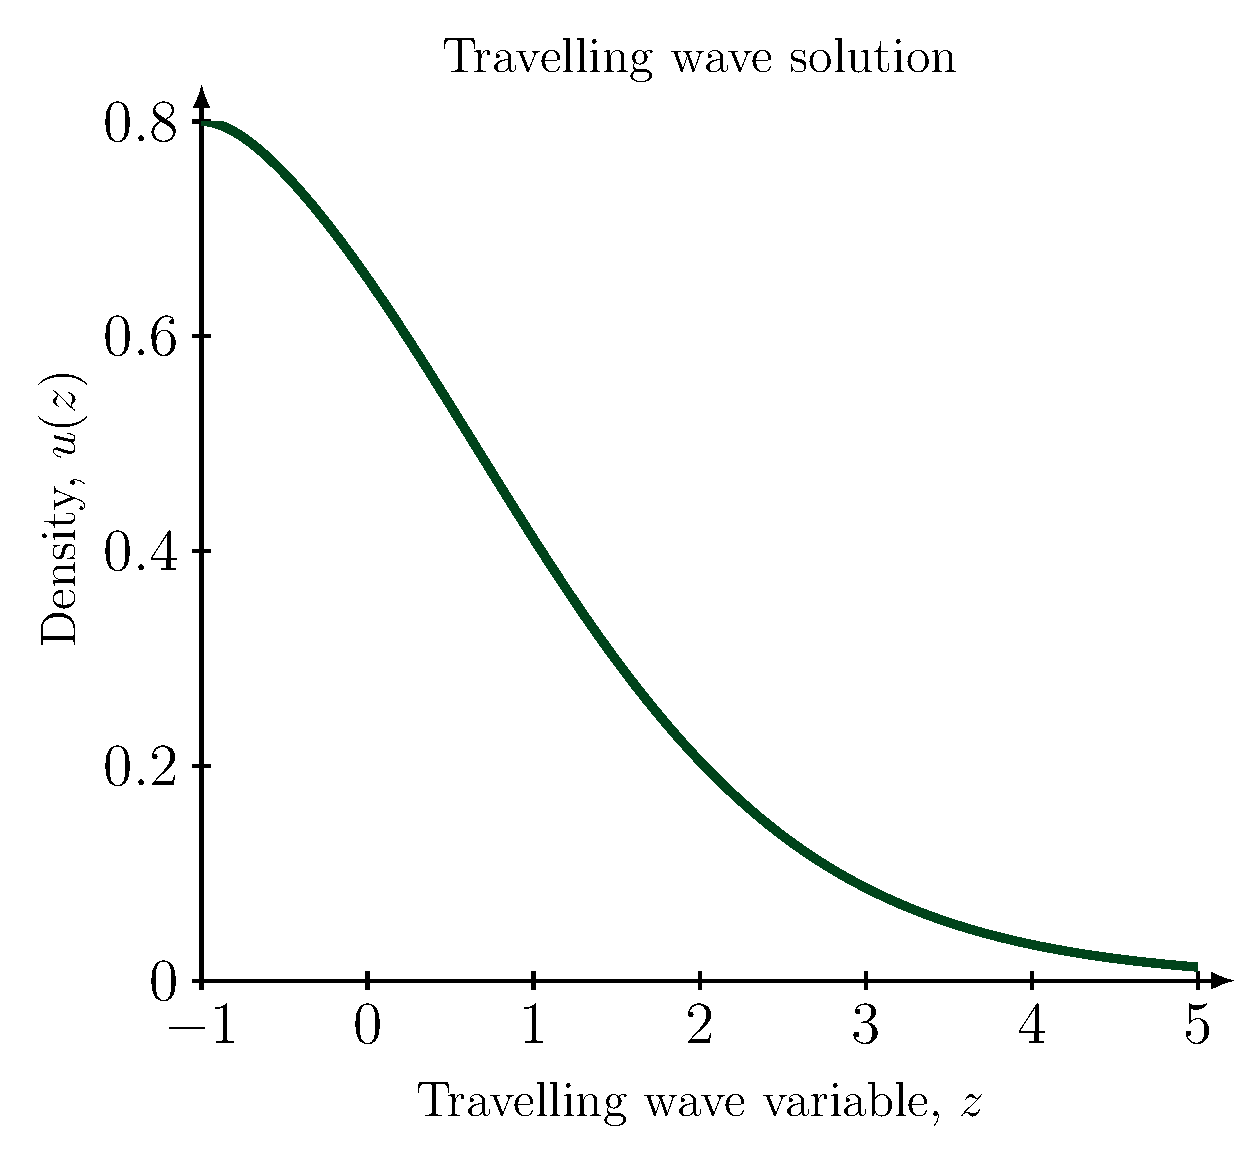
\includegraphics[width=5.0cm,page=1]{{./individual_figures_initial_conditions}}};

\node[inner sep=0pt] (mixed) at (0,0)
{\includegraphics[width=5.0cm,page=2]{{./individual_figures_initial_conditions}}};
\node[inner sep=0pt] (mixed) at (5,0)
{\includegraphics[width=5.0cm,page=3]{{./individual_figures_initial_conditions}}};

% % Vertical lines
%\draw (-7.12,-2.5) -- (-7.12,2.5);
%\draw (-2.12,-2.5) -- (-2.12,2.5);
%\draw (2.88,-2.5) -- (2.88,2.5);
% \draw (2.55,-4.4) -- (2.55,4.7);
% % Horizontal lines
%\draw (-7.8,2.2) -- (7.5,2.2);
% \draw (-7.8,4.43) -- (7.5,4.43);
%\draw (-7.8,2.1) -- (7.5,2.1);
%\draw (-7.8,-2.31) -- (7.5,-2.31);
% Labels of all sub figures
\node (a) at (-6.86,2.33) {(\textbf{A})};
\node[right=4.15cm of a] (b) {(\textbf{B})};
\node[right=4.20cm of b] (c) {(\textbf{C})};


% Add some major axes labels as well
%\node[rotate=90,align=center] (b) at (-7.7,0) {Population density, $u(z)$};
%\node[align=center] (b) at (0,-2.3) {Travelling wave variable, $z$};
% \node[align=center] (b) at (2.5,-2.25) {\scriptsize Prey, $u(t)$};

\end{tikzpicture}

\end{document}

